
\definecolor{dkgreen}{rgb}{0,0.6,0}
\definecolor{gray}{rgb}{0.5,0.5,0.5}
\definecolor{mauve}{rgb}{0.58,0,0.82}

\lstset{frame=tb,
  language=Java,
  aboveskip=3mm,
  belowskip=3mm,
  showstringspaces=false,
  columns=flexible,
  basicstyle={\small\ttfamily},
  numbers=none,
  numberstyle=\tiny\color{gray},
  keywordstyle=\color{blue},
  commentstyle=\color{dkgreen},
  stringstyle=\color{mauve},
  breaklines=true,
  breakatwhitespace=true,
  tabsize=3
}




\chapter{Method of Approach}
\label{ch:method}

\section{Design Overview}
\label{sec:design overview}


The first step to completing the proposed research and to also make sure that everything
would have been accurately accounted for was by first planning out what exactly was necessary
for us to do. Since the topic of this project was to do a SQL injection attack, something that needed to be thought about was what was going to be attacked. SQL injection attacks are typically done against
web-based applications so the plan was to target a web application to do the attack on. After
figuring out that the attack was going to happen to a web application the next step was to think of a specific web application that we could target to properly learn but also
keep in mind that one cannot just perform an attack on any regular web application as that would
not be an ethical thing to do. After talking with my readers, the best option that
we had decided was to create a "dummy" web application as this would allow
me to be able to not only perform a SQL injection but to also have the peace of
mind knowing that if the attack did indeed accidentally made a change to the web application that
there would be harm done to anybody else's work in the process. The framework that was chosen was flask for the creation of this web application. Although there are other options out there
such as Django and streamlit, flask was mostly familiar to me with its design
and also the fact that it uses python as its coding language. Flask also allows for the ability to format the web application and make it look the way we want it to look. The topic
that was chosen for this project isn't common knowledge for everyone so thinking about how others
could navigate when they are on the web application was an important thing to think about. When making the web application it was important to make
the design and layout of the site not only user-friendly but also make sure that
included somewhere on the site a place where the SQL injection could happen. We had chosen
to use a simple layout with not many web pages as this should help people easily
navigate and also understand and follow along with everything that we had decided
to do. We created the site to act as a mock-up for what a banking web application would look like, just to
try and reel in the user and make the illusion that they are actually on a banking
web application with the idea that they are going to inject SQL code to by-pass the
security and gain access to sensitive data. If the user can be engaged to
the fact that they are actually about to try and bypass a login screen by gain access to sensitive information then this project should resonate with them. After all,
everyone who has some sort of money has a bank account, so if we can portray to the user that bypassing login is not quite as difficult as it seems, then
one can believe people will start taking their privacy a lot more seriously. After making
sure we had done everything that we wanted to do and the web application was created, we had
then done the SQL injection attack.


\section{Libraries}
\label{sec:libraries}


When creating the web application using flask, we had to use certain libraries to make sure that we had everything that we needed to ensure that the web application ran properly. we needed to choose ones that would allow me to integrate python with the web application that we needed to create. The first major library that we needed to use in the main program file was, of course, flask. Importing this library would allow me to use the Flask framework and pick a nice template that we could use as a starting point for the web application. The next main library that we needed to use was SQLAlchemy. This library will allow me to create and execute SQL code in the program without having to write SQL statements. For the app file, we needed to import more libraries from flask, but we needed to import specific ones. The ones that we needed to import were render-template, redirect, URL-for, request, and g as well as SQLite3. These specific libraries will allow me first, render the template that we had chosen from flask. Then the redirect library will allow me to redirect the user to a different page if the required requirements were met. The "URL-for" will allow me to redirect the user to a different page using its URL. Request will allow me to ask the user for some type of input. Lastly, g will allow me to connect the database to the web application and have access to it. Using these libraries allowed me to integrate everything that we needed to not only create the flask web application with python but also connect the database to the web application so that the data can be displayed on the web application. Please see Figure ~\ref{fig:web app home page} the web applications interface.


\bigskip
\bigskip
\begin{lstlisting}
from flask import Flask, render_template, redirect, url_for, request, g
import sqlite3
app = Flask(__name__)
app.database = "data.db"
\end{lstlisting}
\bigskip
\bigskip



\bigskip
\bigskip
\begin{figure}[hbt!]
\centering
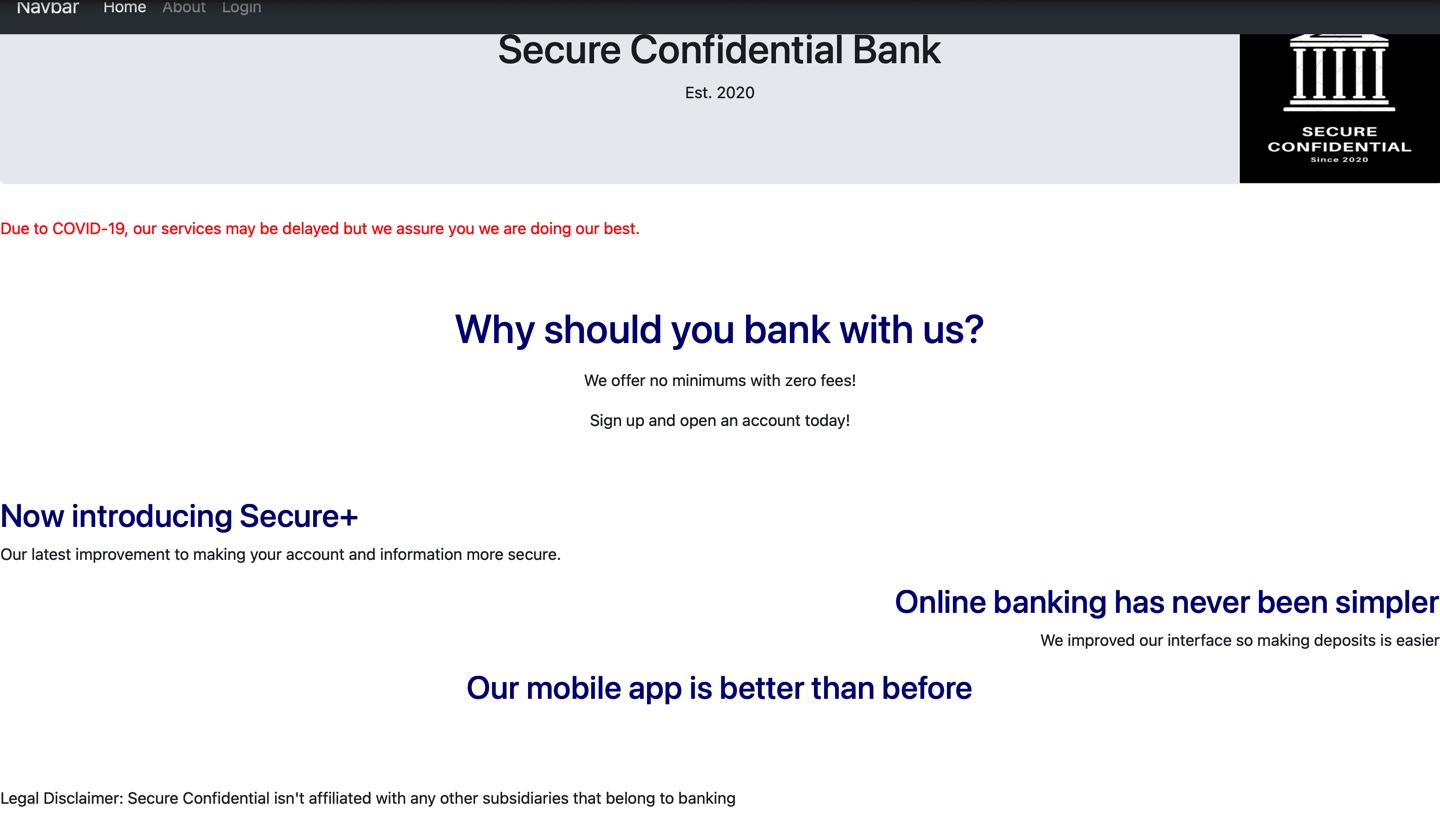
\includegraphics[width=5in]{../images/website.png}%
\caption{Web App Home Page}
\label{fig:web app home page}
\end{figure}

\bigskip
\bigskip


\section{Python Functions}
\label{sec:python functions}

While creating the program in python to create the web application and connect the database, we needed some functions that we could do a few things. First, we needed to create some functions that would allow me to route the links to certain pages on the web application. For example, if we had an about page on the web application, we needed to route the actual about button on the web application to the about page on the web application. The same goes for a home page and the login page. When we talk about the login page though, things can get a little tricky. Once we had routed the login button to the login page, we also needed to route the "success" page that displays all the data within the database but only if one could successfully login. With that being said, we also needed to return the "Invalid" statement if the credentials that one had entered were incorrect. This is where the idea of conditional logic comes in. Conditional logic is simply a set of rules one can place that causes ones process to be changed based on the given input. There are a few different types of conditional logic but here we are just going to focus on one type. The type of conditional logic that we are going to focus on is IF statements. An IF statement simply reads, IF - "this sort of action takes place" then produces this output. What we utilized with the IF statement as well was an else condition. It follows the same pattern as an IF statement. IF - "this sort of action takes place" then produce this output, ELSE - produce this output. You can get the idea of how one can play around with this in programming and that's exactly what we did. we created this thing called a nested loop which allows me to put multiple conditional logic statements within each other. This will allow me to be able to route the "success" page, and the "Invalid" statement if certain conditions were met. All in one function.

\begin{lstlisting}
if username is None:
            error = 'Invalid Credentials. Please try again'
            return render_template('log.html', error=error)
        else:
            return redirect(url_for('hello'))
    else:
        return render_template('log.html', error=error)
\end{lstlisting}

\bigskip
\bigskip

\begin{lstlisting}
@app.route('/')
def home():
    return render_template('home.html')
\end{lstlisting}


\section{HTML and Web Applications}
\label{sec:html and web applications}

When we had created the "dummy" web application and performed the actual SQL injection attack,
we needed to utilize some coding languages as well as databases if we were to properly
and effectively conduct the injection attack. The first coding language
that we had to utilize is HTML. This was imperative because this is the
language that we used while creating the "dummy" web application. HTML simply
stands for hyper-text markup language and this is a web-based language commonly
used when creating a web application. we had decided to use HTML because of its easy-to-understand
language as well as its simplistic syntax. HTML is widely known and used today. Below
is some code from the web application that is in HTML. As one can see, this simply is displaying
text from the about page on the web application.

\bigskip
\bigskip
\begin{lstlisting}



  <div class="jumbotron text-center">
    <h1>About us</h1>
    <p>We are committed to keeping your information secure.</p>
    <image src="{{ url_for('static', filename='images/thesecure.png')}}" width="200" height="180" style="position:absolute; right:-41px; top:43px">
  </div>
    <body>
      <h1><center>Privacy is our top priority</center></h1>
      <p>Here at secure confidential, we pride ourselves on giving our customers world class security to ensure them with the peace of mind knowing that their information is safe and secure. After all, everyone is entitled to have privacy. We can also safely say that we have had zero security issues thus far. Putting your information in someone elses hands is scary, that is why we make it easy to do so. Consider banking with us as we promise your account information is safe and secure.</p>
      <br><br>
      <h2 style="color:navy"><center>Consider these practices when it comes to managing your security</center></h2><br>
      <h3 style="color:red"><center>Regularly change your password</center></h3>
      <p><center>Regularly changing your password will make it harder for others to try and steal your information</center></p><br>
      <h3 style="color:red"><center> Never write down any of your information</center></h3>
      <p><center>Writing down your information could lead to theft</center></p><br>
      <h3 style="color:red"><center> Set up your alerts</center></h3>
      <p><center>Having your alerts on your phone will always allow you to get a notification of transactions in your account in real time</center></p><br>

    </body>




\end{lstlisting}
\bigskip
\bigskip

\section{SQL and Databases}
\label{sec:sql and databases}


The next and important database language that we had to use was SQL. This should not
be a surprise as the title of the thesis is "Assessing vulnerabilities using
SQL injection". We chose SQL because there are a lot of known security issues associated
with SQL and web-based applications. SQL injection is a very common and widely known
technique to attack databases so we wanted to not only see how this was possible
but also figure out why this might be the case and if there are any ways to fix
or mitigate this type of vulnerability. The way we had set up the database though, we had
tried to continue to follow the pattern and idea of how a bank might set up their database.
For simplicity, we had created one database with multiple tables. We can imagine though,
on a much larger scale, there would probably be multiple databases which would make this
process a little more difficult but still, the concept would be the same. The three
tables that we had decided to use were Customers, Managers, and Employees. The way
that we created the database was pretty simple, we decided to use a GUI (graphical user
interface) to set up the columns, rows, and tables in the database because it is a lot
simpler to do it that way, but traditionally, lots of people decide to use the command-line interface for this type of approach. Either way, each option is viable. Please see Figure ~\ref{fig:tables in terminal}.

\bigskip
\bigskip
\begin{figure}[hbt!]
\centering
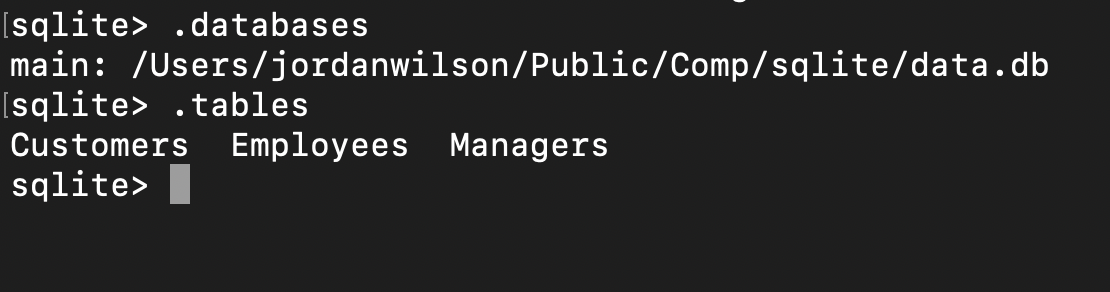
\includegraphics[width=5in]{../images/sql-terminal.png}%
\caption{Tables in terminal}
\label{fig:tables in terminal}
\end{figure}
\bigskip
\bigskip



The next big and important thing that we had to do was to populate the database. We needed
to do this to get all of the data that is not only going to be in
the database but also be displayed on the web application. The approach for doing this was to
simply import a CSV document with lots of fake data. We needed to do this because first,
we obviously could not use real data and second, we wanted a lot of fake data to represent
people and it would take a long time to manually insert all of that data into the
database, not to mention we would have to come up with all of the fake data ourselves, so
we just opted to have a web application generate a lot of fake data and then we were able to import
it. When generating the fake data though, we had to keep in mind the type of
information that we wanted to be displayed in the database. A big proponent of the
project is also the ethics associated with the data that is inside of databases so
we had chosen a bunch of variables that had to show that all of these people have very
private and sensitive information. The types of rows and columns that we had decided to
use were firstname, lastname, age, street, city, state, zip, salary, eye color, dob, religion,
political affiliation, relationship status, and ethnicity. As one can see, a lot of
these factors should not matter to set up a bank account. We had done this to show
that a lot of companies are asking us more information than they need for people
to set up an account with them. This also poses a security issue because if that specific
company has their database breached (which we show in this project) then a lot of people's
sensitive information is shown. Information that does not need to be in a database by some
company. Please see Figure ~\ref{fig:table info}.

\bigskip
\bigskip
\begin{figure}[hbt!]
\centering
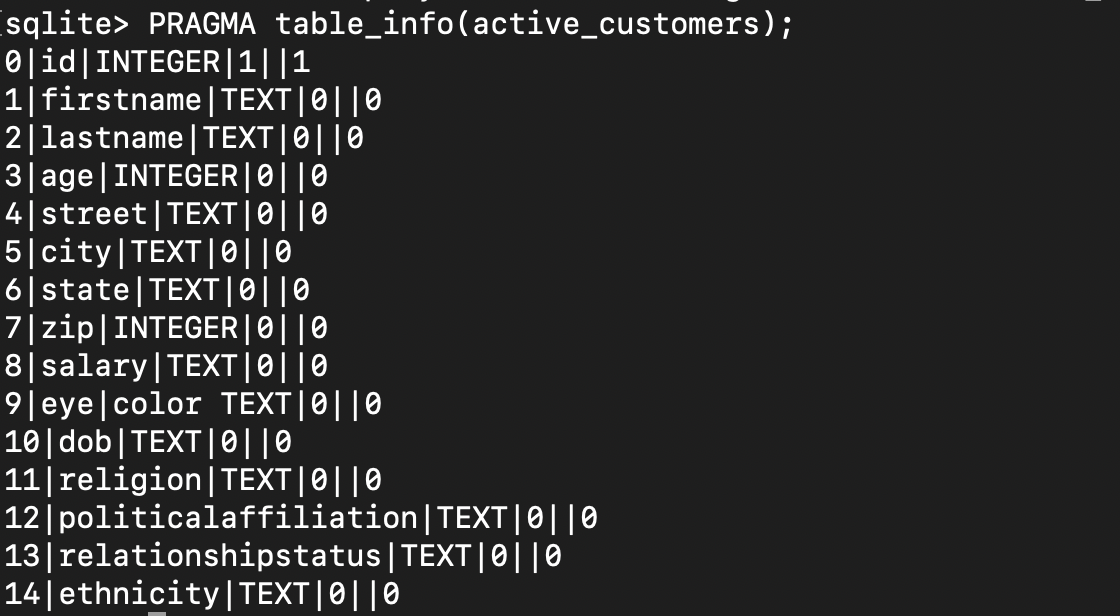
\includegraphics[width=5in]{../images/column-names.png}%
\caption{Table Info}
\label{fig:table info}
\end{figure}
\bigskip
\bigskip

\section{Injection Attack}
\label{sec:injection attack}


When doing the attack, we had to insert SQL queries to try and bypass some
of the log-in administration credentials. With the information that we had gained from
the research of SQL injection attacks, we had done a various number of attacks to try
and inject code into the SQL statements of the web application and gain access to the very sensitive
data that is on the web application. Some examples of things that we did were, we thought
if we were creating a web application, what types of SQL statements would we make to try
and connect the SQL database to the web application to try and make it so that the log-in
credentials would allow someone with the right credentials to log on and see the
information they are allowed to see? When trying to figure out what type of statement
might have been used to connect the database to the site, there were some things that
one could assume were going to be there. First, SELECT username FROM is a good guess as to assuming
what parts of SQL statement would be included since we are dealing with customers and workers
because this is considered to be a banking web application. Stated previously as well, these are also clauses that are common with SQL query statements. Next, we had to try and figure out what may
be on the end of the SQL statement. Well, stated previously, since this is considered to be a banking
web application with log-in credential information, it probably is close to something like, 'username' +
'password'. From here, we can start making some guesses and estimations on what the SQL statement
might look like, but also how we could inject code into this statement to access this data. Again, with the research that we had stated above in the introduction,
there is a lot of common SQL injection code examples that the user could do to bypass a log-in.
With this knowledge, we then started trying different common SQL queries to
gain access. Low and behold, one of the techniques that we had ended up trying actually
worked. This piece of code worked simply because of what it is saying in the SQL query statement. The piece of code was " OR 1=1 --. This worked mainly because of what we were doing. We set the statement to automatically be true. 1=1 is a true statement but the OR in the statement nullifies the SQL query that is proceeding with the statement that we injected. The way it works is like this, imagine we have some sort of random SQL query statement: "SELECT * FROM blah blah blah WHERE blah blah. What we did was we injected SQL code at the end of this query so it would read like this: "SELECT * FROM blah blah blah WHERE blah blah OR 1=1." Ultimately this is negating the first part of the SQL query because the injection is setting everything equal to true. Please see Figure ~\ref{fig:injection attack}

\bigskip
\bigskip
\begin{figure}[hbt!]
\centering
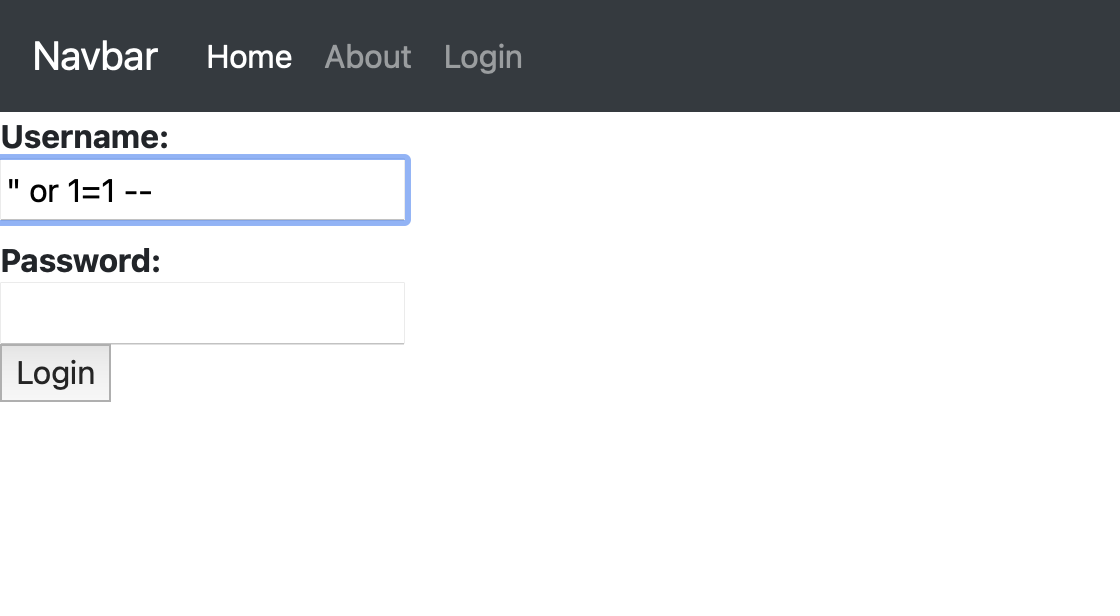
\includegraphics[width=5in]{../images/sql-injection1.png}%
\caption{Injection attack}
\label{fig:injection attack}
\end{figure}
\bigskip
\bigskip

\section{Prototype Implementation}
\label{sec:prototype implementation}


After the SQL injection attack and time permitting, we then started the implementation
for a prototype that allows for better security involving databases. The two main services that we used to help create the prototype were first cloud computing. As we have learned, cloud computing will help with security measures because, cloud computing will allow for the database to not statically sit
on a dedicated server or machine, but it will allow for the database to be accessed
through the cloud. The next service or prototype that we used to implement the prototype was a VPN. From the related work articles, we believed using a VPN helped
with privacy and security as well as it scrambles users' IP addresses and location services so
that the user wouldn't be tracked.

When it comes to the VPN and Cloud computing component of the project, we had to make
sure we could use some sort of software that would allow us to integrate both prototypes.
With much research on this topic, we then concluded using Algo VPN
and digitalOcean cloud computing software. These two prototypes allowed us to set up
a "firewall" of sorts that created an extra layer of security. With the AlgoVPN data
structure, we could create the server and watch and monitor traffic on that
dedicated server ourselves. If anyone tries to access that specific server, we will be
notified. When we paired this with the digitalOcean cloud computing infrastructure, the user will
then be forced to log in to the cloud to access the very sensitive data that
is inside of the database. When the user puts this all together, this is how it should look
like. The first step to access this vital sensitive information would to first
fire up the AlgoVPN and connect to a specific server so that only the user could monitor
the traffic (I.E., no one else knowing where the user is logging onto the database from).
Next, the user can log in to the digitalOcean cloud computing platform and put in the users credentials (
assuming the user has "rights" to view this database). From there, the user should be able to
see the vital information that the user does not want other people to see.


\section{VPN Creation}
\label{sec:vpn creation}


To first start with the implementation of the prototype, we had to first figure
out how to set up the VPN using Algo. With algo, there is a lot of customization.
For starters though, to get going, the user will need to just first download the
required software to do so. We found the documentation from trailofbits.com
And from here we were able to get started. After the user follows the directions, to get
all of the required packages on the users machine up and running one will then need to start up
their virtual environment. For me, I had to go into the algo directory,
then go into the myenv directory, then to the bin directory, and once here, I simply just typed
'source activate' and I was able to start up the virtual environment and get everything running
and underway. Please see Figure ~\ref{fig:virtual environment}

\bigskip
\bigskip
\begin{figure}[hbt!]
\centering
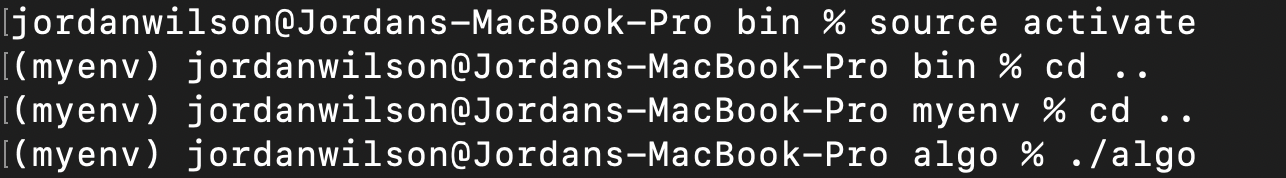
\includegraphics[width=5in]{../images/myenv-1.png}%
\caption{Virtual Environment}
\label{fig:virtual environment}
\end{figure}
\bigskip
\bigskip



After we can get the virtual environment up and running, the next thing we need to
do is start up the algo program to create the VPN. To do that
we simply just type './algo' and the user will then be prompted with a bunch of questions.
The first question that they ask is which cloud provider one would like to use. we had decided
to use DigitalOcean but there are other options such as Amazon EC2, Openstack, Cloudstack,
and others as well. Please see Figure ~\ref{fig:cloud provider}

\bigskip
\bigskip
\begin{figure}[hbt!]
\centering
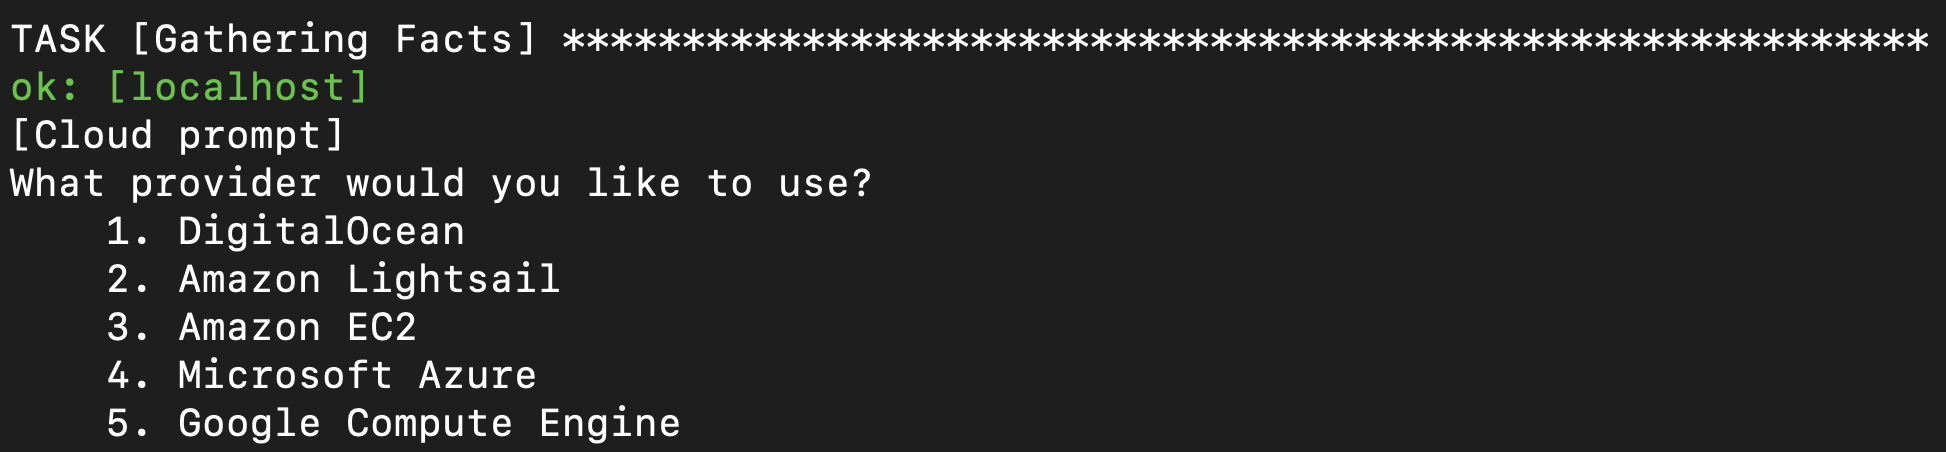
\includegraphics[width=5in]{../images/provider-1.png}%
\caption{Cloud Provider}
\label{fig:cloud provider}
\end{figure}
\bigskip
\bigskip




After the user has chosen which provider they had decided to go with, it then asks the user
a bunch of questions about how to set up the server. It's going to ask the user things
such as VPN server name, if the user wants it to be enabled on clients on-demand for wifi and
cellular networks, names of any trusted wifi networks if one wants to retain any PKI keys,
If the user want to enable DNS blocking on this server, and if the user wants each user of the VPN to have their own
SSH tunneling. From there, it is going to download a few things and then ask the user for their API
token. From there the user will have the option to choose the location of the server, and once that
is down, the user has finally created a VPN. Please see Figure ~\ref{fig:vpn success}



\bigskip
\bigskip
\begin{figure}[hbt!]
\centering
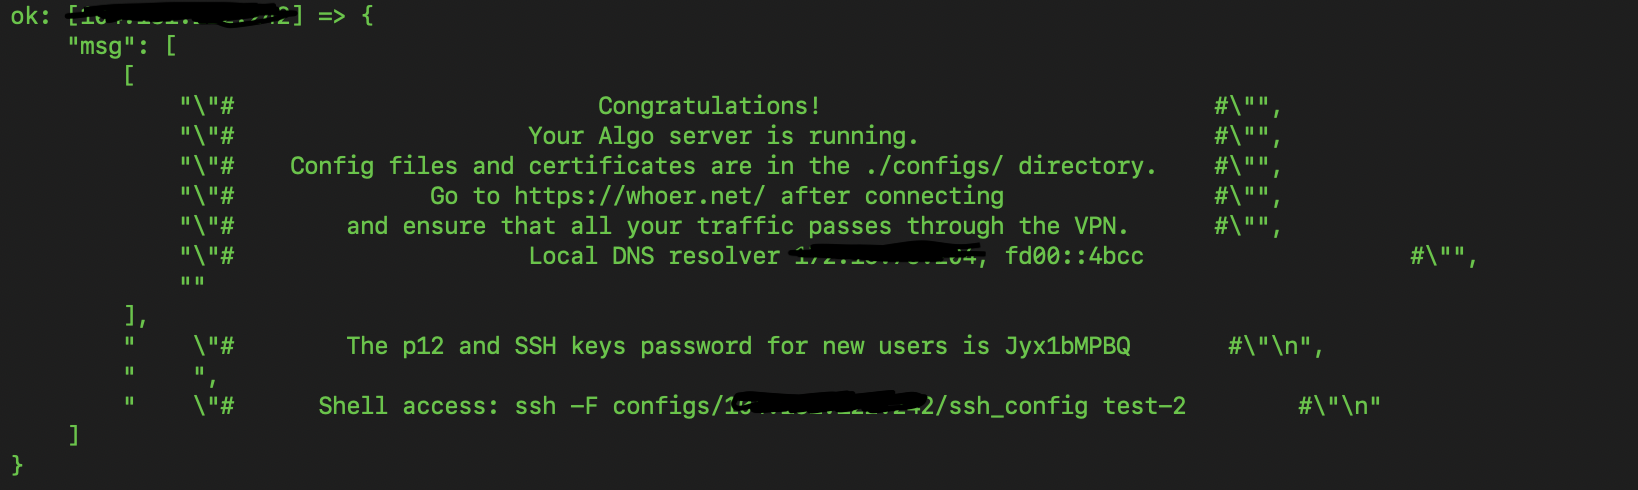
\includegraphics[width=5in]{../images/algo-success1.png}%
\caption{VPN Success}
\label{fig:vpn success}
\end{figure}
\bigskip
\bigskip



From here we now have to access our newly configured VPN. There are a few options available
to us to do that. The options that we have are phone, tablet, and laptop. Personally,
I had decided to set it up on my phone. Once we are greeted with the congratulations
page that our VPN is set up, it also gives us a web application that we have to go to to make sure our new IP address is masked. The web application is whoer.net and we'll just keep
this there for reference right now. To use the VPN on a device, we
have to have wireguard VPN installed. This will allow us to connect to our server. Once we have
wireguard installed, it will let us add a new connection at the top right of the screen.
From there, we can name our new connection and then actually connect to it. There are two different
ways the user can connect to the server through wireguard, but the easiest way and the way that we did
it was to simply use the barcode that is in our algo files. This will allow for easy
connectivity for us to connect to the server. Once we had located the phone barcode
picture, we then just went back on my phone and scanned the barcode and we then were
easily able to connect to the VPN server! After we had done this, we then went
back to the whoer.net web application we had referenced earlier and we were able to see that I
was connected to a different server and the IP address was indeed masked. Please see Figure ~\ref{fig:vpn access}



\bigskip
\bigskip
\begin{figure}[hbt!]
\centering
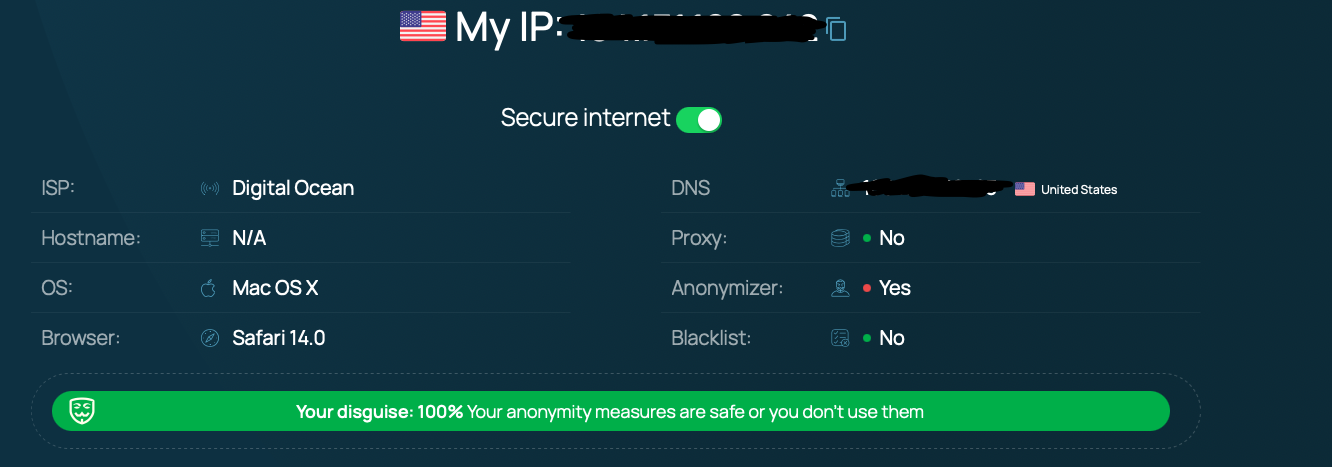
\includegraphics[width=5in]{../images/whoer-1.png}%
\caption{VPN Access}
\label{fig:vpn access}
\end{figure}
\bigskip
\bigskip
\bigskip
\bigskip


\section{Cloud Database Cluster}
\label{sec:cloud database cluster}


After the completion of the VPN server, we now could move onto creating the cloud virtual
server to create a database and access it. For this part, we used DigitalOcean
almost exclusively. The first big step we did to create the databases through
DigitalOcean was that we needed to purchase a database cluster from DigitalOcean.
With DigitalOcean, there come subscriptions that the user will have to pay for to
use their services which is unfortunate, but their services do make what we were trying to
do a bit easier. After we had purchased a database cluster, we then start picking and choosing
what options we am going to need. In digitalOcean there are a few different engines the user can
use. The options are PostgreSQL, MySQL, and Redis. For this project, we decided to
use Redis. The next option the user has is how large one would want their node size to be. For this
option though, the user has to be careful because the bigger the node size, the more money
they will have to pay a month for this cluster. The next thing the user has to choose is
a data center. For convenience, we decided to go with New York since that is close to where
we am and it will take less time connecting to the database cluster but other options
the user can choose from are Amsterdam, San Francisco, London, and Singapore just to name a few.
After the user has chosen their desired settings, all one has to do now is come up with a unique
database cluster name. Please see Figure ~\ref{fig:mysql connection}



\bigskip
\bigskip
\bigskip

\bigskip
\begin{figure}[hbt!]
\centering
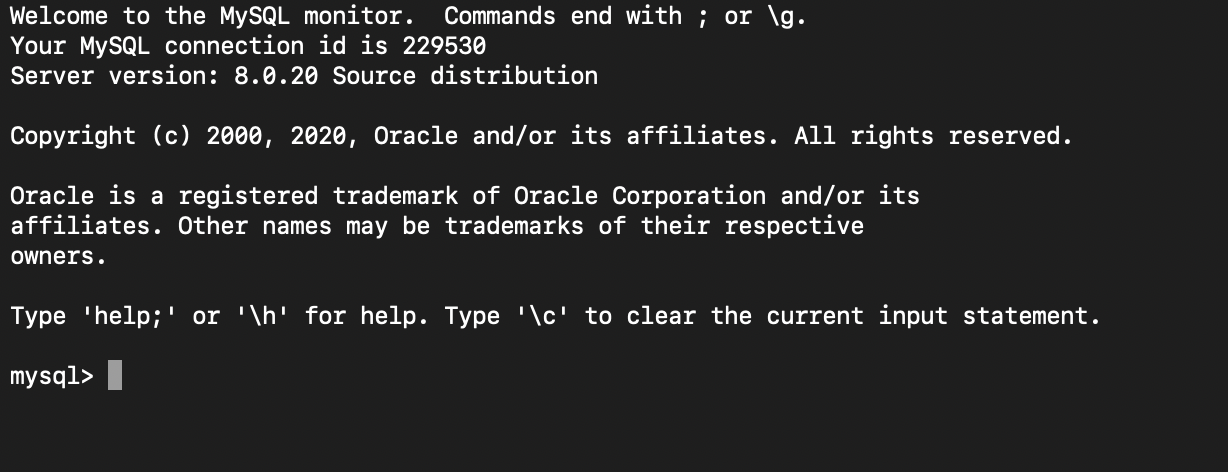
\includegraphics[width=5in]{../images/mysql-terminal.png}%
\caption{MySQL Connection}
\label{fig:mysql connection}
\end{figure}
\bigskip




After the creation of the users database cluster, one has to set some preferences as well.
A big preference one has to set is their trusted sources. This is super vital to this
project. This is how we will integrate the VPN and the database cluster. What I
did was I set the trusted sources to only it being the VPN IP that we had created earlier.
With this, I am able to only access this database cluster when I am connected to a specific
VPN server that I (or the user) have created. This just adds an extra layer of security.
After the user chooses their trusted sources and fill out the rest of the information that one
would like, digitalOcean will provide the user with their connection parameters, and from here
one can connect to the database cluster. Please see Figure ~\ref{fig:mysql databases cluster}


\bigskip
\bigskip

\begin{figure}[hbt!]
\centering
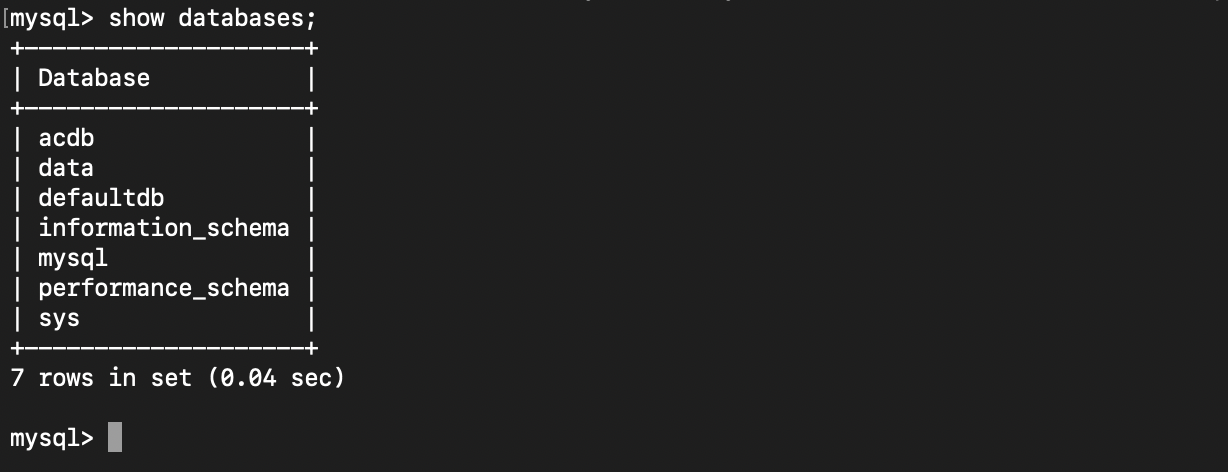
\includegraphics[width=5in]{../images/mysql-db.png}%
\caption{MySQL Databases Cluster}
\label{fig:mysql databases cluster}
\end{figure}





